% 图 60.2 —— 由 `checks/emit_hand.py` 自动拼出（probe 精测 + prims2 图元分解）
%%
% ⚠ 这是**稿子不是成品**：跑 `checks/checkhand.py 60.2` 看指标 + 看叠合图。
%%
%% ⚠ 待核：
%   · 本图 probe 报出阴影族 1 个 —— **本脚本不生成阴影**（要照原书手写）；prims2 的 strokes 里可能含阴影线，核对时留意别画重
%   · 可疑字形 2 项（空心圈 ⊙ 常被认成字母 o）—— 见文件末
%%
\documentclass[12pt]{standalone}
\usepackage{fontspec}
\setsansfont{Arial}
\newfontfamily\mfallback{DejaVu Sans}
\usepackage{tikz}
\begin{document}
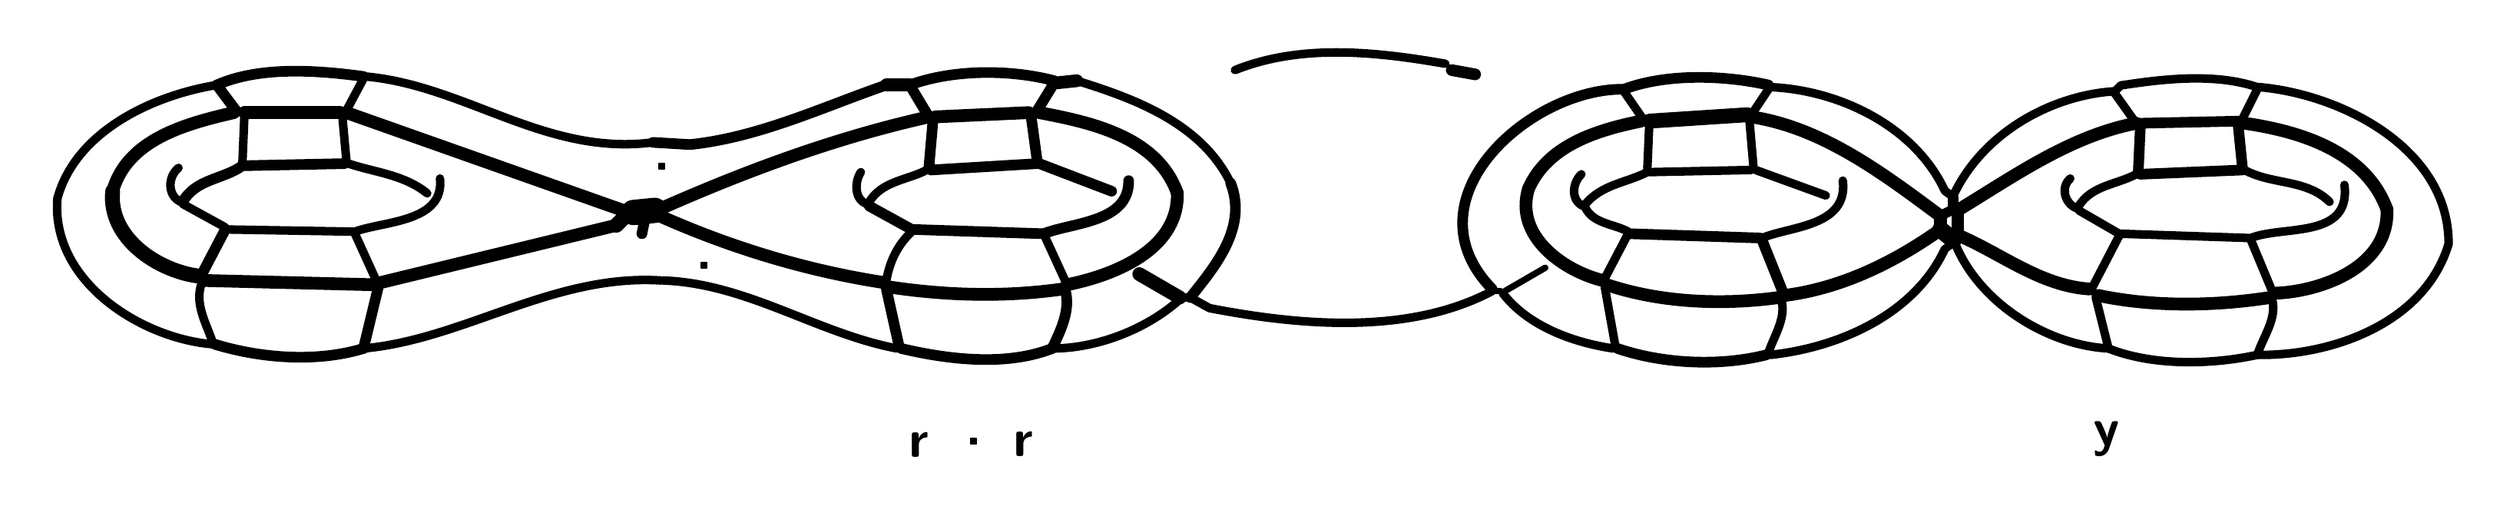
\begin{tikzpicture}[x=1pt, y=-1pt, line width=5.1pt, line cap=round, line join=round]

  %% ════ 直线段（prims2 的 strokes）════
  \draw[line width=5.1pt] (297.0,91.0) -- (293.0,94.0);
  \draw[line width=3.0pt] (717.0,116.0) -- (698.0,127.0);
  \draw[line width=6.0pt] (418.0,30.0) -- (407.0,30.0);
  \draw[line width=5.0pt] (418.0,30.0) -- (427.0,45.0);
  \draw[line width=5.0pt] (478.0,66.0) -- (475.0,44.0);
  \draw[line width=4.0pt] (974.0,126.0) -- (987.0,101.0);
  \draw[line width=6.0pt] (903.0,98.0) -- (903.0,92.0);
  \draw[line width=7.9pt] (903.0,98.0) -- (909.0,103.0);
  \draw[line width=6.5pt] (545.0,130.0) -- (526.0,119.0);
  \draw[line width=5.0pt] (757.0,100.0) -- (818.0,102.0);
  \draw[line width=5.0pt] (513.0,80.0) -- (479.0,67.0);
  \draw[line width=4.0pt] (815.0,69.0) -- (813.0,46.0);
  \draw[line width=4.0pt] (849.0,82.0) -- (816.0,70.0);
  \draw[line width=4.0pt] (559.0,135.0) -- (550.0,130.0);
  \draw[line width=4.0pt] (1052.0,32.0) -- (1045.0,46.0);
  \draw[line width=6.0pt] (430.0,45.0) -- (474.0,43.0);
  \draw[line width=5.0pt] (314.0,58.0) -- (297.2,57.0);
  \draw[line width=4.0pt] (988.0,100.0) -- (1048.0,102.0);
  \draw[line width=4.0pt] (745.0,121.0) -- (756.0,100.0);
  \draw[line width=4.0pt] (153.0,66.0) -- (151.0,44.0);
  \draw[line width=4.0pt] (153.0,42.0) -- (161.0,27.0);
  \draw[line width=5.0pt] (96.0,98.0) -- (85.0,119.0);
  \draw[line width=4.0pt] (763.0,46.0) -- (754.0,33.0);
  \draw[line width=5.0pt] (413.0,153.0) -- (407.0,126.0);
  \draw[line width=3.0pt] (696.0,127.0) -- (693.0,127.0);
  \draw[line width=6.0pt] (153.0,43.0) -- (286.0,90.0);
  \draw[line width=4.0pt] (968.0,89.0) -- (987.0,100.0);
  \draw[line width=5.0pt] (161.0,154.0) -- (168.0,125.0);
  \draw[line width=7.0pt] (286.0,90.0) -- (280.0,96.0);
  \draw[line width=6.0pt] (280.0,96.0) -- (169.0,123.0);
  \draw[line width=4.0pt] (492.0,124.0) -- (481.0,100.0);
  \draw[line width=5.0pt] (1044.0,47.0) -- (997.0,48.0);
  \draw[line width=5.0pt] (429.0,46.0) -- (427.0,69.0);
  \draw[line width=5.0pt] (486.0,29.0) -- (478.0,42.0);
  \draw[line width=4.0pt] (765.0,70.0) -- (766.0,47.0);
  \draw[line width=3.8pt] (908.0,105.0) -- (905.0,107.2);
  \draw[line width=11.9pt] (288.0,90.0) -- (298.0,89.0);
  \draw[line width=4.0pt] (167.0,122.0) -- (157.0,100.0);
  \draw[line width=5.0pt] (420.0,98.0) -- (481.0,100.0);
  \draw[line width=5.0pt] (819.0,103.0) -- (829.0,128.0);
  \draw[line width=4.0pt] (985.0,34.0) -- (995.0,48.0);
  \draw[line width=5.0pt] (399.0,87.0) -- (419.0,98.0);
  \draw[line width=5.0pt] (152.0,67.0) -- (104.0,68.0);
  \draw[line width=5.0pt] (292.0,100.0) -- (293.0,95.0);
  \draw[line width=7.0pt] (812.0,44.0) -- (766.0,47.0);
  \draw[line width=4.0pt] (156.0,99.0) -- (97.0,98.0);
  \draw[line width=4.7pt] (908.0,89.0) -- (904.0,91.0);
  \draw[line width=5.5pt] (673.0,23.0) -- (684.0,25.0);
  \draw[line width=4.0pt] (76.0,86.0) -- (96.0,97.0);
  \draw[line width=6.0pt] (105.0,43.0) -- (150.0,43.0);
  \draw[line width=4.0pt] (104.0,68.0) -- (105.0,44.0);
  \draw[line width=4.0pt] (546.0,130.0) -- (550.0,130.0);
  \draw[line width=4.0pt] (987.8,30.2) -- (985.0,33.0);
  \draw[line width=4.0pt] (905.0,79.8) -- (908.0,82.0);
  \draw[line width=5.0pt] (1045.0,69.0) -- (1043.0,49.0);
  \draw[line width=4.0pt] (976.0,130.0) -- (982.0,154.0);
  \draw[line width=4.0pt] (1059.0,127.0) -- (1049.0,103.0);
  \draw[line width=4.0pt] (814.0,44.0) -- (822.0,32.0);
  \draw[line width=5.0pt] (909.0,83.0) -- (909.0,88.0);
  \draw[line width=5.2pt] (292.0,94.0) -- (288.0,91.0);
  \draw[line width=4.0pt] (766.0,71.0) -- (814.0,70.0);
  \draw[line width=5.0pt] (101.0,42.0) -- (92.0,30.0);
  \draw[line width=5.0pt] (478.0,67.0) -- (428.0,70.0);
  \draw[line width=6.0pt] (911.0,100.0) -- (911.0,90.0);
  \draw[line width=6.0pt] (487.0,29.0) -- (496.6,28.0);
  \draw[line width=6.0pt] (86.0,122.0) -- (166.0,124.0);
  \draw[line width=5.0pt] (996.0,71.0) -- (997.0,49.0);
  \draw[line width=5.0pt] (997.0,72.0) -- (1045.0,70.0);
  \draw[line width=4.0pt] (750.0,153.0) -- (745.0,125.0);

  %% ════ 曲线（prims2 的 curves —— 三段式，坐标同为 (y,x)）════
  \draw[line width=4.0pt] (756.0,99.0) .. controls (749.4,95.4) and (739.8,95.3) .. (736.0,88.0);
  \draw[line width=5.0pt] (418.0,30.0) .. controls (438.4,22.6) and (465.0,22.5) .. (486.0,28.0);
  \draw[line width=5.0pt] (407.0,30.0) .. controls (376.7,40.5) and (347.4,54.5) .. (315.0,58.0);
  \draw[line width=6.0pt] (1046.0,48.0) .. controls (1071.6,51.7) and (1103.0,61.0) .. (1113.0,88.6);
  \draw[line width=6.0pt] (1113.0,88.6) .. controls (1114.1,115.6) and (1082.1,127.3) .. (1060.0,128.0);
  \draw[line width=4.0pt] (90.0,152.0) .. controls (56.8,149.3) and (13.9,122.8) .. (17.0,83.4);
  \draw[line width=4.0pt] (17.0,83.4) .. controls (25.7,51.5) and (62.3,34.8) .. (92.0,30.0);
  \draw[line width=6.0pt] (903.0,98.0) .. controls (881.1,113.5) and (856.7,125.5) .. (830.0,129.0);
  \draw[line width=4.0pt] (571.0,23.0) .. controls (602.1,10.5) and (637.4,14.3) .. (670.0,20.0);
  \draw[line width=4.0pt] (692.0,127.0) .. controls (652.9,147.7) and (601.8,143.3) .. (559.0,135.0);
  \draw[line width=6.0pt] (299.0,91.0) .. controls (332.8,106.2) and (368.9,117.3) .. (406.0,123.0);
  \draw[line width=6.0pt] (299.0,89.0) .. controls (340.2,70.7) and (382.9,54.8) .. (427.0,45.0);
  \draw[line width=4.0pt] (1093.0,77.0) .. controls (1096.2,102.8) and (1064.0,95.9) .. (1049.0,102.0);
  \draw[line width=4.0pt] (157.0,99.0) .. controls (170.5,94.0) and (199.2,94.7) .. (197.0,74.0);
  \draw[line width=4.0pt] (297.2,57.0) .. controls (246.9,63.6) and (209.0,30.2) .. (162.0,26.0);
  \draw[line width=4.0pt] (545.0,131.0) .. controls (529.1,145.2) and (505.9,154.0) .. (485.0,154.0);
  \draw[line width=4.0pt] (75.0,85.0) .. controls (68.7,82.1) and (68.8,73.2) .. (74.0,69.0);
  \draw[line width=6.0pt] (814.0,45.0) .. controls (847.1,50.1) and (875.1,71.0) .. (902.0,91.0);
  \draw[line width=4.0pt] (412.0,154.0) .. controls (374.3,146.8) and (341.5,123.4) .. (302.0,122.0);
  \draw[line width=5.0pt] (751.0,154.0) .. controls (772.1,161.2) and (798.9,162.6) .. (821.0,157.0);
  \draw[line width=6.0pt] (911.0,89.0) .. controls (937.7,72.8) and (964.0,54.0) .. (995.0,48.0);
  \draw[line width=6.0pt] (746.0,124.0) .. controls (771.1,132.4) and (800.0,133.7) .. (827.0,130.0);
  \draw[line width=4.0pt] (1059.0,131.0) .. controls (1061.4,139.9) and (1054.6,148.7) .. (1052.0,157.0);
  \draw[line width=5.0pt] (161.0,154.0) .. controls (139.1,160.7) and (112.5,158.6) .. (91.0,152.0);
  \draw[line width=4.0pt] (161.0,154.0) .. controls (208.4,149.7) and (250.2,118.8) .. (301.0,122.0);
  \draw[line width=4.0pt] (697.0,128.0) .. controls (708.9,143.5) and (730.1,151.2) .. (749.0,154.0);
  \draw[line width=6.0pt] (492.0,124.0) .. controls (513.5,119.7) and (544.6,107.8) .. (543.9,80.9);
  \draw[line width=6.0pt] (543.9,80.9) .. controls (534.4,54.2) and (503.1,47.6) .. (479.0,43.0);
  \draw[line width=4.0pt] (964.0,74.0) .. controls (959.2,78.2) and (961.5,85.9) .. (967.0,88.0);
  \draw[line width=6.0pt] (1058.0,130.0) .. controls (1031.8,134.1) and (1002.8,134.5) .. (977.0,129.0);
  \draw[line width=4.0pt] (1046.0,70.0) .. controls (1058.6,77.0) and (1075.2,74.2) .. (1086.0,85.0);
  \draw[line width=4.0pt] (399.0,85.0) .. controls (404.8,75.2) and (417.2,74.7) .. (426.0,70.0);
  \draw[line width=4.0pt] (984.0,33.0) .. controls (953.5,35.3) and (922.4,53.4) .. (909.0,82.0);
  \draw[line width=4.0pt] (905.0,107.2) .. controls (890.5,138.3) and (854.7,153.6) .. (823.0,157.0);
  \draw[line width=5.0pt] (491.0,126.0) .. controls (494.0,135.6) and (489.0,145.5) .. (485.0,154.0);
  \draw[line width=4.0pt] (419.0,99.0) .. controls (412.2,105.2) and (408.5,113.3) .. (407.0,122.0);
  \draw[line width=5.0pt] (692.0,126.0) .. controls (651.1,84.0) and (709.3,32.1) .. (753.0,32.0);
  \draw[line width=5.0pt] (822.0,30.0) .. controls (801.1,25.3) and (773.9,24.5) .. (754.0,32.0);
  \draw[line width=4.0pt] (828.0,131.0) .. controls (830.6,139.5) and (824.6,148.1) .. (822.0,156.0);
  \draw[line width=5.0pt] (104.0,68.0) .. controls (95.2,74.4) and (81.9,74.2) .. (76.0,85.0);
  \draw[line width=4.0pt] (1052.0,31.0) .. controls (1032.3,24.4) and (1008.4,27.0) .. (987.8,30.2);
  \draw[line width=4.0pt] (823.0,31.0) .. controls (855.4,32.4) and (890.9,49.4) .. (905.0,79.8);
  \draw[line width=4.0pt] (857.0,75.0) .. controls (859.6,96.7) and (832.3,96.4) .. (819.0,102.0);
  \draw[line width=4.0pt] (154.0,67.0) .. controls (166.5,71.2) and (180.2,72.2) .. (191.0,81.0);
  \draw[line width=6.0pt] (912.0,101.0) .. controls (931.9,109.6) and (950.2,124.5) .. (973.0,126.0);
  \draw[line width=4.0pt] (968.0,87.0) .. controls (973.8,77.3) and (986.1,76.8) .. (995.0,72.0);
  \draw[line width=5.0pt] (521.0,75.0) .. controls (521.3,94.9) and (494.3,94.6) .. (481.0,100.0);
  \draw[line width=5.0pt] (414.0,154.0) .. controls (436.1,159.2) and (463.3,162.5) .. (485.0,154.0);
  \draw[line width=4.0pt] (398.0,86.0) .. controls (391.8,84.1) and (392.0,75.5) .. (395.0,71.0);
  \draw[line width=6.0pt] (408.0,125.0) .. controls (435.0,129.1) and (462.7,129.9) .. (490.0,126.0);
  \draw[line width=6.0pt] (100.0,43.0) .. controls (78.5,48.0) and (49.9,55.2) .. (43.0,80.0);
  \draw[line width=7.0pt] (43.0,80.0) .. controls (40.8,102.2) and (64.7,117.8) .. (84.0,120.0);
  \draw[line width=4.0pt] (736.0,86.0) .. controls (743.5,76.8) and (755.3,76.0) .. (765.0,71.0);
  \draw[line width=4.0pt] (735.0,87.0) .. controls (728.8,84.5) and (729.7,76.0) .. (734.0,72.0);
  \draw[line width=4.0pt] (1052.0,157.0) .. controls (1030.0,161.8) and (1002.6,162.2) .. (982.0,154.0);
  \draw[line width=4.0pt] (1052.0,157.0) .. controls (1086.9,157.6) and (1130.8,142.2) .. (1142.0,104.8);
  \draw[line width=4.0pt] (1142.0,104.8) .. controls (1142.2,59.8) and (1091.5,34.4) .. (1053.0,31.0);
  \draw[line width=6.0pt] (762.0,47.0) .. controls (742.2,51.1) and (718.3,57.9) .. (709.1,78.9);
  \draw[line width=6.0pt] (709.1,78.9) .. controls (702.4,101.1) and (725.5,117.4) .. (744.0,122.0);
  \draw[line width=4.0pt] (90.0,151.0) .. controls (87.2,142.4) and (81.2,132.8) .. (85.0,123.0);
  \draw[line width=4.0pt] (910.0,105.0) .. controls (921.7,133.2) and (953.7,152.5) .. (982.0,154.0);
  \draw[line width=5.0pt] (92.0,30.0) .. controls (112.0,21.1) and (139.1,23.0) .. (161.0,26.0);
  \draw[line width=4.0pt] (496.6,28.0) .. controls (523.8,36.4) and (555.3,48.0) .. (569.0,76.2);
  \draw[line width=5.0pt] (569.0,76.2) .. controls (577.0,96.9) and (562.0,115.0) .. (550.0,130.0);

  %% ════ 标签（probe 直接给的 \node 行）════
  %% ⚠ 全部补了 fill=white：文字在最上层，否则与曲线交叉干扰
     \node[anchor=center,inner sep=0pt,fill=white,font=\fontsize{41.1}{51.3}\selectfont] at (301.6,68.3) {\textsf{\textbf{.}}};   % box(296,65,5,6)
     \node[anchor=center,inner sep=0pt,fill=white,font=\fontsize{30.0}{37.5}\selectfont] at (321.2,115.2) {\textsf{\textbf{.}}};   % box(317,113,4,4)
     \node[anchor=center,inner sep=0pt,fill=white,font=\fontsize{30.7}{38.3}\selectfont] at (981.3,196.3) {\textsf{\textbf{\textit{y}}}};   % box(972,183,18,23)
     \node[anchor=center,inner sep=0pt,fill=white,font=\fontsize{41.4}{51.7}\selectfont] at (422.4,199.4) {\textsf{\textbf{\textit{r}}}};   % box(411,186,18,22)
     \node[anchor=center,inner sep=0pt,fill=white,font=\fontsize{81.3}{101.6}\selectfont] at (448.1,197.7) {\textsf{\textbf{.}}};   % box(435,186,14,22)
     \node[anchor=center,inner sep=0pt,fill=white,font=\fontsize{40.2}{50.3}\selectfont] at (471.8,199.3) {\textsf{\textbf{\textit{r}}}};   % box(461,186,17,22)

  % 钉死画布：否则超出的图元/控制点会把页面撑大，1:1 回比就失准
  \pgfresetboundingbox
  \path[use as bounding box] (0,0) rectangle (1156,218);
\end{tikzpicture}
\end{document}

% ⚠ 待核清单（probe 拿不准，人眼过一遍）：
%   · 未识别/跳过：⑤ 跳过/未识别的字形
%   · 未识别/跳过：box(318,70,5,5)
